\chapter{Tecnologías más eficientes. Captura de $\textbf{CO}_2$.}
\section{Evolución de las calderas de combustión de carbón.}
Las calderas de carbón pulverizado se dividen en:
\begin{itemize}
	\item [-] Subcríticas: eficiencia del 35\% PCI.
	\item [-] Supercríticas o ultracríticas: eficiencia del 40\% PCI. 
	\begin{itemize}
		\item Presión > 248 bar
		\item Temperatura > 566\grado
		\item Emite menos CO$_2$ que las subcríticas
	\end{itemize}
\end{itemize}
Las tecnologías limpias por su parte han avanzado para que se elimine gran parte de los gases emitidos.
\begin{itemize}
	\item [-] Precipitadores electrostáticos y filtros: Eliminan el 99\% de la ceniza. 
	\item [-] Métodos de desulfuración: Eliminan el 90-97\% de los SO$_x$.
	\item [-] Quemadores de bajo NO$_x$ y técnicas de requemado: Reducen los NO$_x$ un 50\%.
	\item [-] Reducción catalítica postcombustión: Reducen los NO$_x$ un 80-90\%.
\end{itemize}
El desarrollo de las calderas ultrasupercríticas de carbón pulverizado supone un problema de resistencia térmica y mecánica de los materiales. 
\begin{itemize}
	\item [-] Tubos de conducción del vapor vivo a temperaturas > 600 \grado.
	\item [-] Aumento del grosor de las paredes de los tubos por aumentar la presión.
\end{itemize}
\subsection{Turbina de vapor.}
Clásicamente las turbinas de vapor han trabajado con el foco caliente a 170 bar y 540\grado con un rendimiento del 36\%.


Actualmente para soportar los ciclos supercríticos se necesitan turbinas más robustas para soportar en el foco caliente 310 bar y 567\grado $\ $  con un rendimiento del 42\%.
\newpage
\section{Tecnología de captura y almacenamiento de CO$_2$.}
\begin{figure}[H]
	\centering
	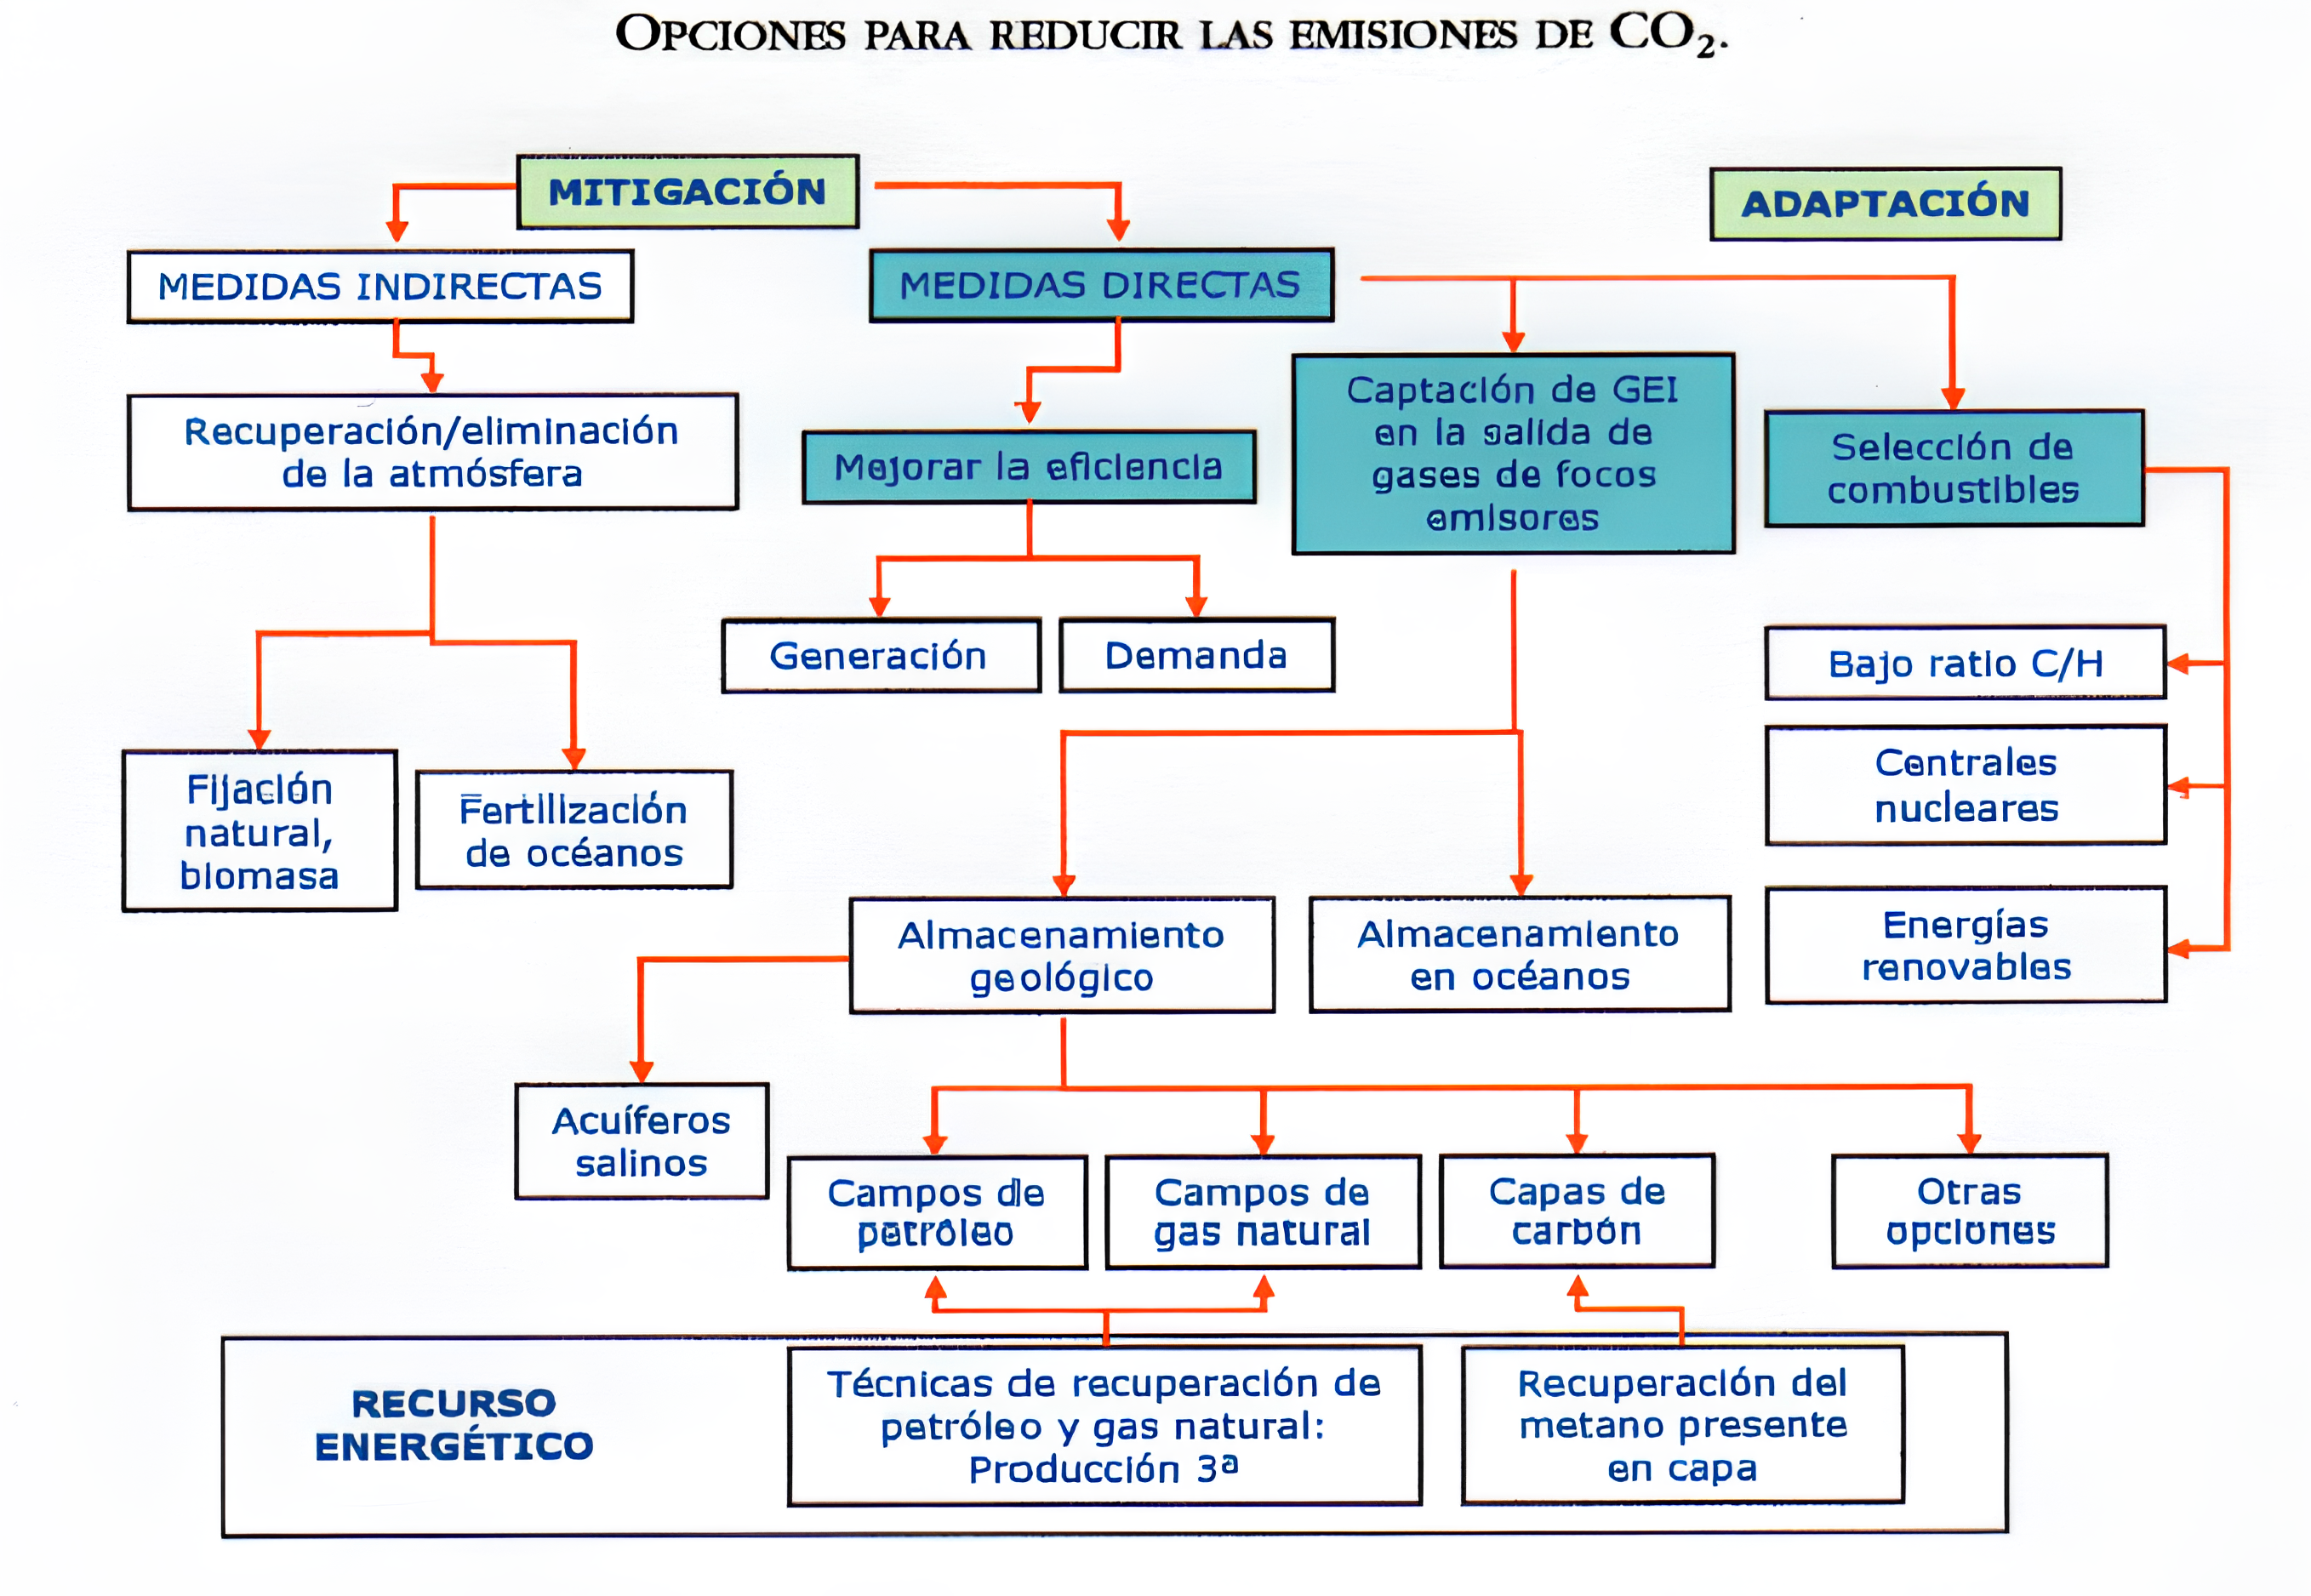
\includegraphics[width=0.7\linewidth]{res/tema3/reduccionCO2Opt}
	\label{fig:reduccionco2opt}
\end{figure}

\subsection{Combustión convencional del carbón pulverizado.}
Una planta de 500 MW eléctricos consume alrededor de 200 t/hora de carbón y entre
2000 y 2100 t/hora de aire (nitrógeno y oxígeno). Esta planta emite por cada 100 kg de gases efluentes están compuestos aproximadamente por 71 kg de
nitrógeno, 21 kg de CO$_2$, 3 kg de agua y 4 kg de oxígeno.

Por tanto, es necesario separar el CO$_2$ y no permitir que salga a la atmósfera para procesarlo. En función de la tecnología empleada se reduce una cantidad de CO$_2$ emitido distinto.
\begin{itemize}
	\item [-] Reducción del 18\% en calderas supercríticas.
	\item [-] Reducción del 30\% en calderas ultrasupercríticas.
	\item [-] Reducción del 90\% en calderas CAC (captura y almacenamiento CO$_2$).
\end{itemize}
\begin{figure}[H]
	\centering
	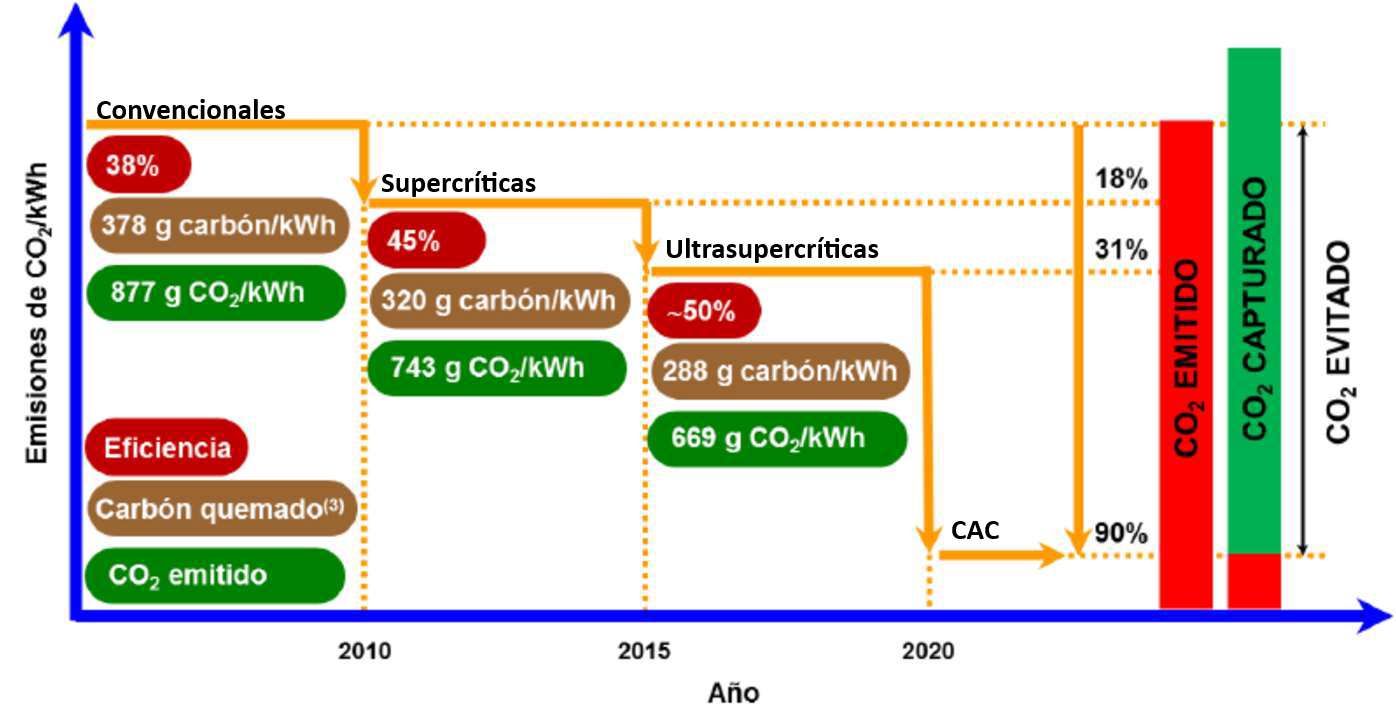
\includegraphics[width=0.7\linewidth]{res/tema3/comparacion calderas}
	\label{fig:comparacion-calderas}
\end{figure}

\subsection{Co-combustión.}
La co-combustión consiste en utilizar biomasa mezclada con el carbón pulverizado. Esto permite moderar el impacto mediambiental ya que la biomasa tiene bajo contenido en S, N, Hg y CO$_2$. A su vez, también permite reducir la temperatura de los gases a la salida del hogar y controlar los inquemados.
\begin{itemize}
	\item [-]\textbf{Co-combustión directa:}
	Se puede realizar mediante inyección premezclada (<2\%) o inyección separada (5-10\%) a un coste de 100-140€/kWe.
	
	\item [-]\textbf{Co-combustión indirecta:}
	Se sintetiza biogas como sustituto del combustible y conlleva un coste de 800€/kWe.
\end{itemize}
Se comprueba experimentalmente que añadir biomasa mejora el rendimiento de la caldera y, además, reduce la cantidad de NO$_x$ emitidos porque el proceso de volatilización es más rápido.
\begin{figure}[H]
	\centering
	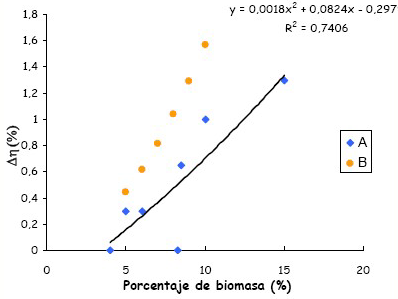
\includegraphics[width=0.5\linewidth]{res/tema3/influenciaBiomasa}
	\label{fig:influenciabiomasa}
\end{figure}

\subsection{Captura CO$_2$ antes de la combustión.}
Para reducir la cantidad de CO$_2$ emitido se gasifica el combustible con oxígeno para obtener un gas de síntesis que contiene CO y H$_2$. A continuación se hace reaccionar el CO con agua para generar más H$_2$ y CO$_2$ (Es una tecnología muy unida a la producción de hidrógeno).

La principal ventaja de esta opción es que el CO$_2$ se encuentra concentrado a alta presión lo que permite emplear métodos de separación más eficiente.


La principal desventaja es que se requiere de una planta de fraccionamiento de aire(ASU) que tiene unos costes y consumo energético elevados.
\begin{figure}[H]
	\centering
	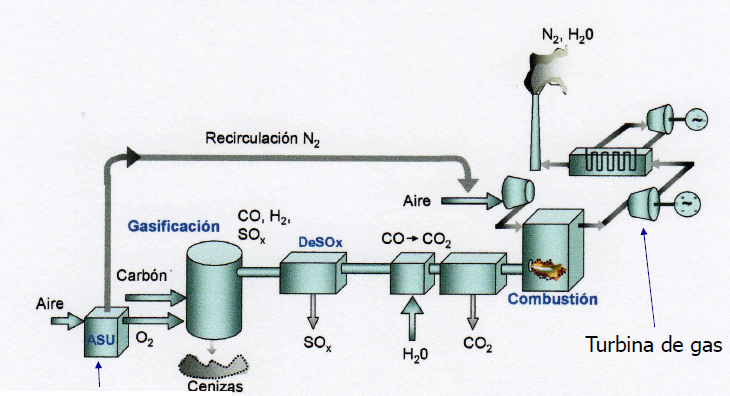
\includegraphics[width=0.7\linewidth]{res/tema3/ASU}
	\label{fig:asu}
\end{figure}

\subsection{Captura CO$_2$ durante la combustión.}
Para capturar el CO$_2$ durante la combustión se emplea la técnica de oxicombustión que consiste en realizar la combustión directamente con oxígeno en ausencia de nitrógeno.


Para poder llevar a cabo este proceso, es necesario emplear una ASU (consumo de 220kWh/t CO$_2$).Los gases de combustión generados serán fundamentalmente CO$_2$ y H$_2$O, los cuales son fácilmente
separables, obteniendo un CO$_2$ de elevada pureza, que puede ser llevado a la unidad de compresión y
dejarlo listo para su transporte y almacenamiento.


La principal ventaja de esta tecnología es su bajo coste 30€/t de CO$_2$. 


El principal inconveniente es que los gases alcanzan la tenperatura de 2550\grado durante la combustión y para evitarlo se recirculan los gases húmedos (CO$_2$) a una temperatura más baja.
\subsection{Captura CO$_2$ tras la combustión.}
Para capturar el CO$_2$ existen varias técnicas:
\begin{enumerate}
	\item \textbf{Absorción química:}
		Es el proceso más utilizado industrialmente.Este, consiste en hacer pasar los gases por una columna que contiene sorbente líquido que capta el CO$_2$ (90\% capturado) que posteriormente en una etapa de regeneración se libera el CO$_2$ para su transporte y se recircula el sorbente. 
		
		Los reactivos utilizados en los procesos de absorción química están basados en disoluciones acuosas de
		alcanolaminas.
		
		Las principales ventajas de esta tecnología son:
		\begin{itemize}
			\item Modificaciones menores en las centrales.
			\item Se puede emplear en serie para optimizar el proceso.
			\item Permite tratar un volumen alto de gases.
		\end{itemize}
		Aunque tiene el inconveniente de que las impurezas de NO$_x$ y SO$_x$ afectan al sistema.
	\item \textbf{Absorción física:}
		El proceso se desarrolla a alta presión haciéndolo un sistema viable en procesos de combustible gasificado. Para realizar la separación los gases se ponen en contacto con un solvente orgánico en una torre de absorción.
	\item \textbf{Adsorción:}
		Se emplean tamices moleculares o carbón activo. Aún no se comercializa la tecnología.
	\item \textbf{Membranas:}
		El proceso comercial utiliza una membrana de polímeros para separar el gas, lo cual tiene como
		consecuencia un mayor consumo de energía que en un proceso estándar de absorción química.
	\item \textbf{Carbonatación o calcinación:}
		Se emplea caliza para hacerla reaccionar con el CO$_2$ y así retirarlo de manera sencilla (debe incorporarse un sistema de recuperación de la caliza).
		\[CaO+CO_2\rightarrow CaCO_3+1800kJ/kg\]
\end{enumerate}
\subsection{Transporte y almacenamiento de CO$_2$.}
Tras la captura y compresión del CO$_2$ se transporta y almacena. El transporte se realiza a través de tuberías o barcos en fase supercrítica o líquida.
\begin{figure}[H]
	\centering
	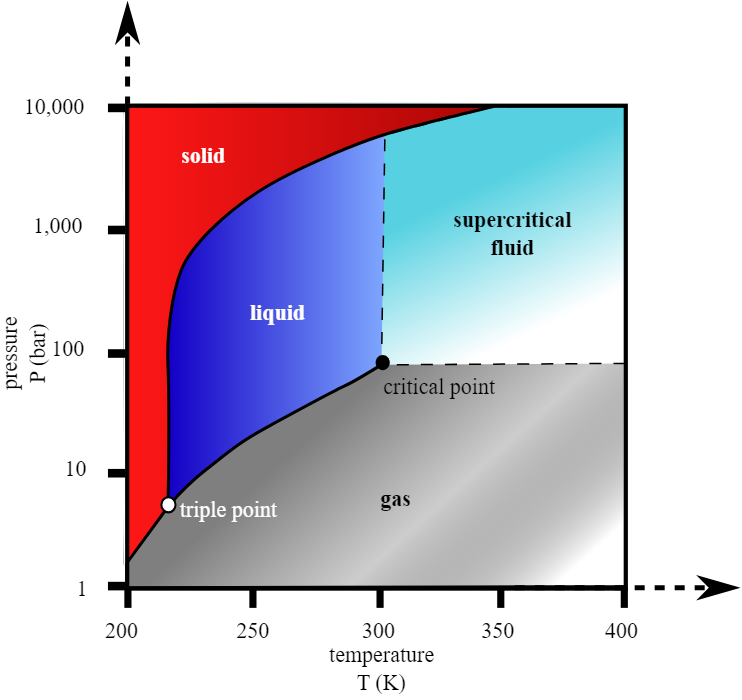
\includegraphics[width=0.4\linewidth]{res/tema3/triple}
	\label{fig:triple}
\end{figure}
Para almacenar el CO$_2$ normalmente se emplean formaciones geológicas, es decir, se inyecta el CO$_2$ bajo tierra bien en formaciones geológicas salinas (sin utilidad para el consumo humano) o en yacimientos de petróleo y así sacar más hidrocarburo.
\begin{figure}[H]
	\centering
	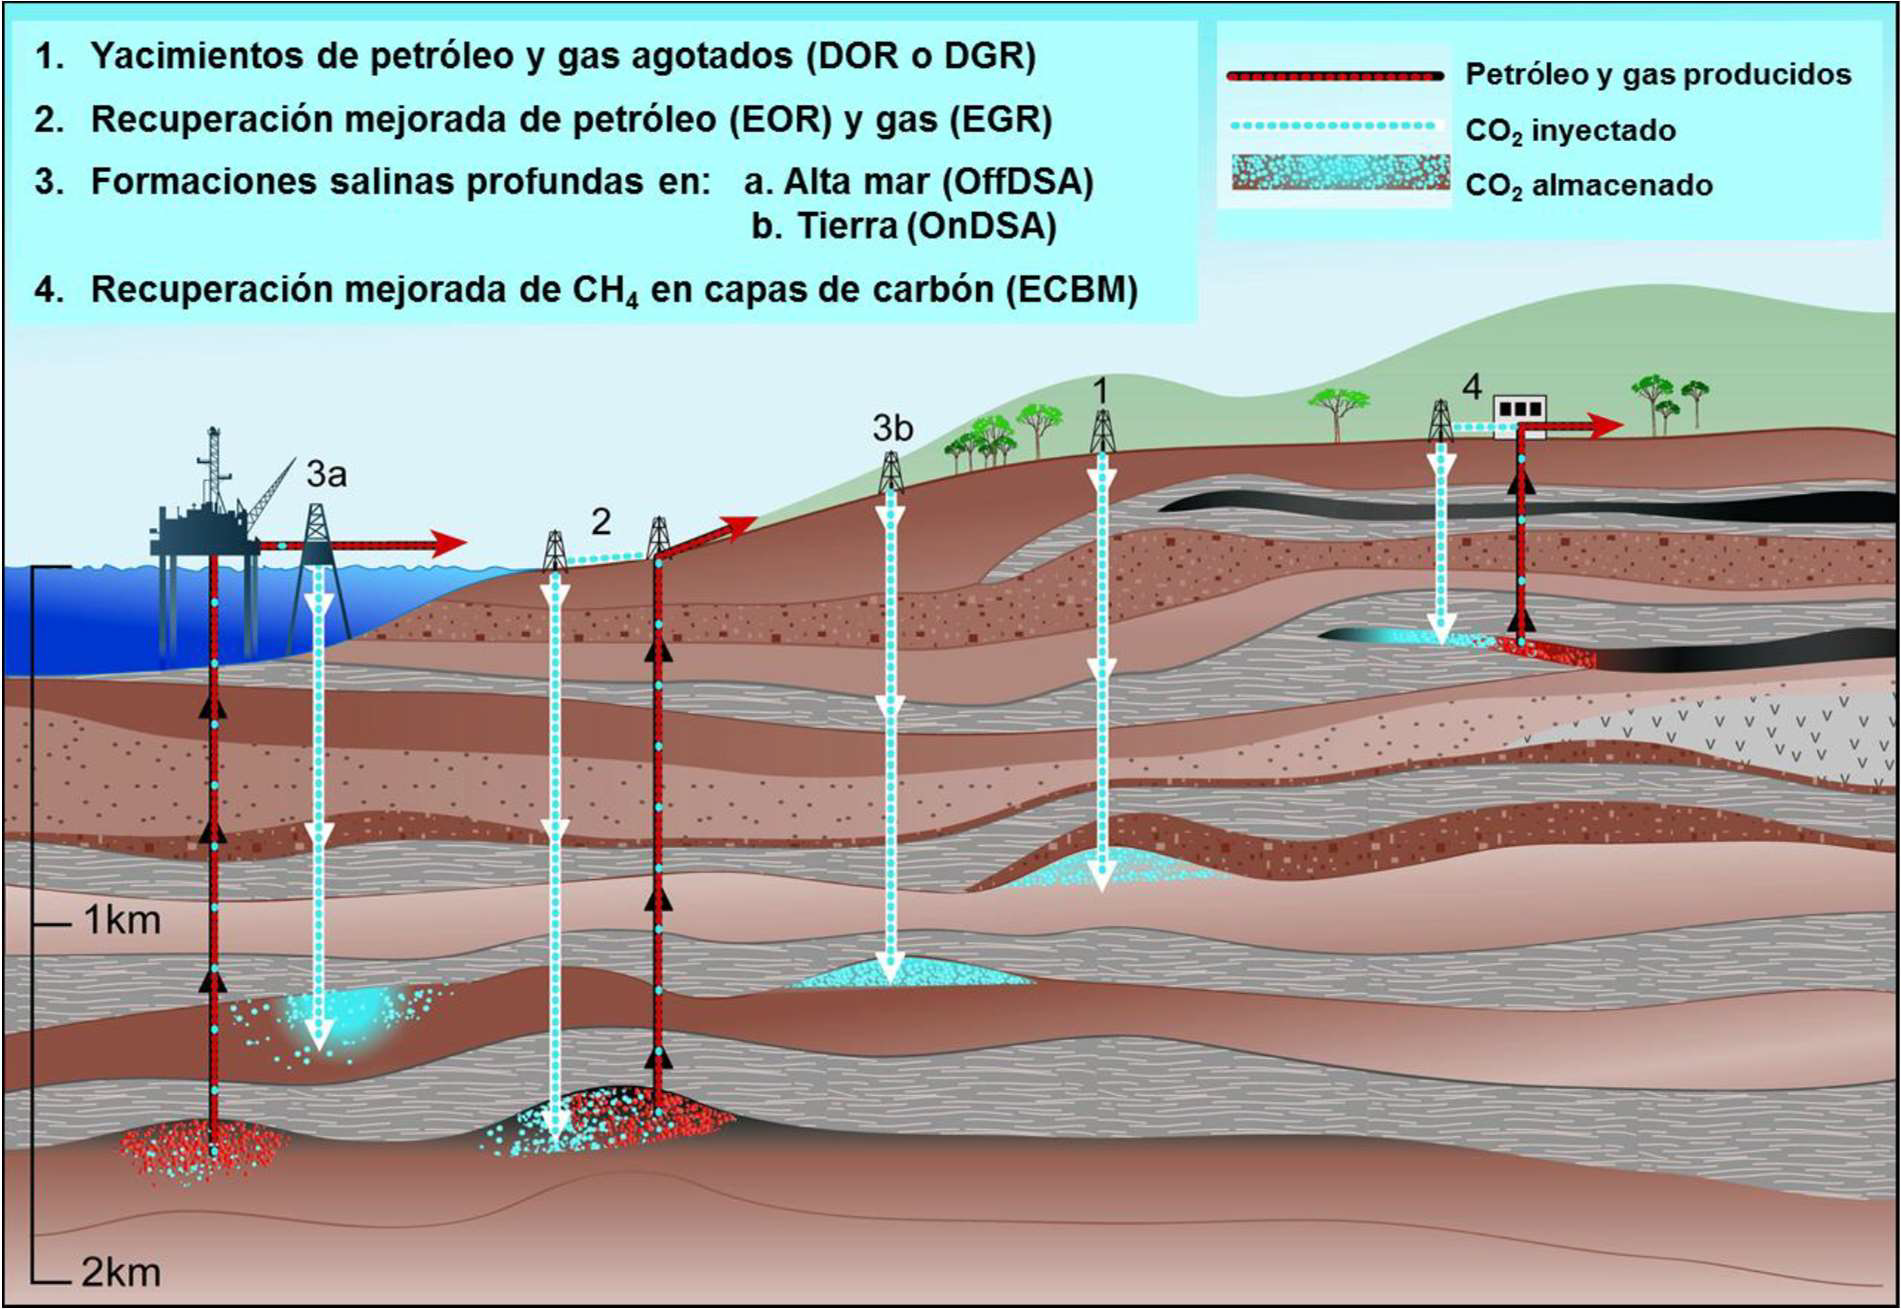
\includegraphics[width=0.5\linewidth]{res/tema3/almacen1}
	\label{fig:almacen1}
\end{figure}

\subsection{Transformación CO$_2$ en metano.}
Con el CO$_2$ capturado y añadiendo hidrógeno se puede obtener metano que puede ser empleado como sustituto del gas natural en la red gasista. 
\[CO_2+3H_2\rightarrow CH_4+2H_2O\]
Otra alternativa es la obtención de biometanol a través del CO$_2$ mediante la digestión anaerobia de los residuos orgánicos.
\[CO_2+3H_2\xrightarrow{catalizador} CH_3OH+H_2O\]
\section{Calderas de combustión de lecho fluidizado (CLF).}
Se desarrollan debido a que permiten reducir las emisiones así como permitir quemar combustibles de bajo poder calorífico. Actualmente, alcanzan potencias unitarias de 300MWe.

El lecho fluido se consigue al hacer pasar un fluido (aire) en dirección ascendente a través de un lecho de partículas sólidas inértes con tamaño entre los 0,5-3 mm. En este lecho se introduce carbón triturado en partículas de 5-10 mm.

Menos del 2\% del material del lecho es el combustible. El resto son cenizas y absorbente (caliza) para absorber el azufre y formar CaSO$_4$ (yeso). Además, el lecho se enfria por intercambiadores de manera que las temperaturas se mantienen en el rango 800-900\grado.
\subsection{Ventajas CLF.}
\begin{itemize}
	\item \textbf{Comportamiento similar a un fluido:}
		Permite que los sistemas de alimentación, eliminación de cenizas y automatización sean relativamente sencillos.
	\item \textbf{Distribución temperaturas uniforme:}
		Debido a que el combustible se comporta como un fluido el control es sencillo y se evita que se queme el nitrógeno del aire. \textbf{No se forman NO$_x$}.
	\item \textbf{Desulfuración:}
		Como se introducen absorbentes el SO$_2$ es capturado por la caliza y no se libera al aire. La temperatura ideal para máxima absorción es la de 850\grado.
	\item \textbf{Admite diversidad de combustibles.}
	\item \textbf{Alta difusividad del aire de combustión:}
		Como la granulometría es baja hay elevada superficie de contacto y por tanto, la reacción es más rápida.
	\item \textbf{Alta transferencia de calor:}
		Suele ser del orden de unas cien veces mayor que en las calderas de lecho
		estático con carbón pulverizado. Esto, permite que se monte el intercambiador de calor (agua-vapor) en el seno del lecho.
	\item \textbf{No se forman escorias:}
		Como la temperatura no supera los 850\grado las cenizas no funden y son fáciles de retirar.
	\item \textbf{Menor exceso del aire de combustión:}
		Se debe a que la reacción es más favorable por la superficie de contacto.
\end{itemize}
\newpage
\subsection{Tipos de CLF.}
Según la velocidad del aire de fluidización:
\begin{enumerate}
	\item \textbf{Lecho fluido estacionario o burbujeante (CLFB):}
		Con bajas velocidades de fluidificación del aire (3m/s) menos del 10\% de los sólidos pasan al ciclón. Eficiencia de combustión del 93\%.
	\begin{figure}[H]
		\centering
		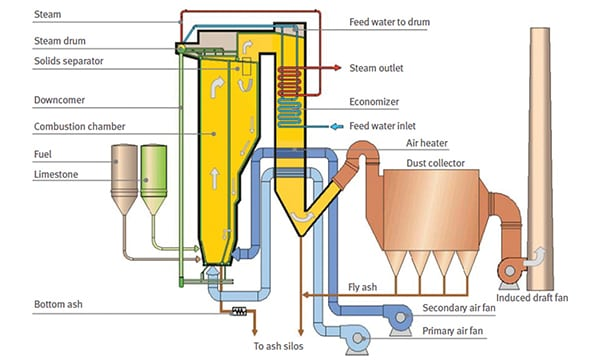
\includegraphics[width=0.7\linewidth]{res/tema3/clfb}
		\label{fig:clfb}
	\end{figure}
	
	\item \textbf{Lecho fluido circulante (CLFC ):}
			Con elevadas velocidades de fluidificación del aire (8m/s) se arrastra un gran número de sólidos que pueden reciclarse mediante un ciclón. Eficiencia de combustión del 98\%.
	\begin{figure}[H]
		\centering
		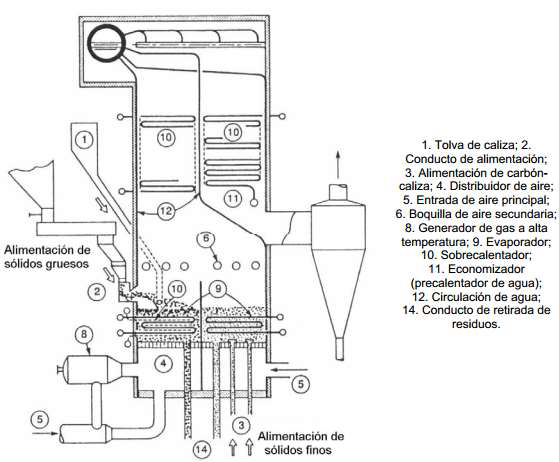
\includegraphics[width=0.7\linewidth]{res/tema3/CLFC}
		\label{fig:clfc}
	\end{figure}
	
\end{enumerate}
Según la presión a la que se realice el proceso:
\begin{enumerate}
	\item \textbf{Lechos atmosféricos:} Necesitan más caliza para retener el azufre.
	\item \textbf{Lechos presurizados:} Trabajan con presiones en torno a los 16 bar. Tienen un rendimiento superior al 40\%. Fijan mejor el azufre y emiten menos NO$_x$. Tienen menor coste pero desgastan más la superficie de caldeo.
\end{enumerate}
\newpage
\section{Gasificación del carbón.}
La gasificación es un proceso termoquímico en el cual la energía en un combustible sólido se transfiere a los productos primarios del proceso (gases, líquidos y hollín) de los cuales el más interesante es el gas de síntesis (75\% PC del carbón).

Este proceso emplea un agente gasificante y tiene lugar a temperaturas elevadas 800\grado.
\begin{table}[H]
	\centering
	\begin{tabular}{p{3cm}p{3cm}p{3cm}p{3cm}}
		\toprule
		Gasificación&Clase de gas&Componentes&Aplicación \\
	 	\midrule
	 	Con aire y vapor				&Gas combustible (<6MJ/Nm$^3$)							& Oxígeno, carbono, hidrógeno y nitrógeno& Combustible en la industria\\
	 	Con aire y vapor a presión		&Gas combustible (<6MJ/Nm$^3$)							&Oxígeno, carbono, hidrógeno, nitrógeno y metano&Gas para centrales \\
	 	Con oxígeno y vapor				&Gas de síntesis y de reducción (10-20MJ/Nm$^3$)		&Oxígeno, carbono e hidrógeno& Industria química \\
	 	Con oxígeno y vapor a presión	&Gas natural (>30MJ/Nm$^3$)	y gas ciudad (poco usado)	&Hidrógeno y metano& Suministro público \\
		\bottomrule
	\end{tabular}
	\label{tab:4x5_table}
\end{table}

\subsection{Tipos de gasificadores.}
\begin{itemize}
	\item [-] Reactores de lecho móvil o fijo en updraft: Sistemas de pequeña escala (8MW).
	\item [-] Reactores de lecho móvil o fijo en downdraft: Sistemas de pequeña escala (8MW).
	\item [-] Reactores de lecho fluidizado: Sistemas de media escala.
	\item [-] Reactores lecho arrastrado a presión.
\end{itemize}
\begin{figure}[H]
	\centering
	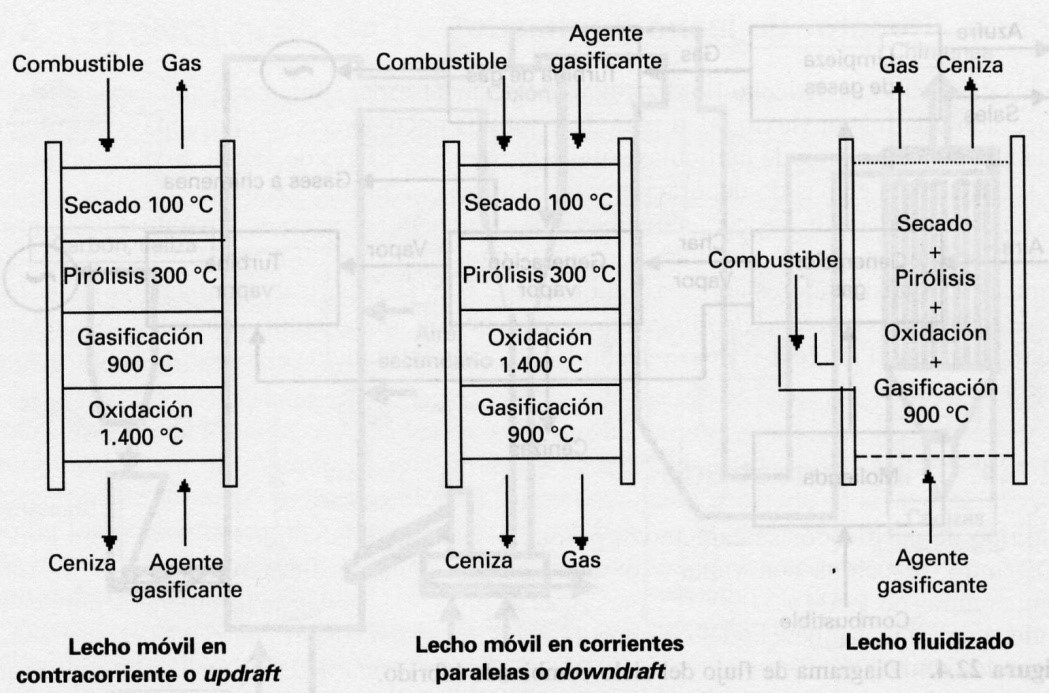
\includegraphics[width=0.7\linewidth]{res/tema3/gasificad}
	\label{fig:gasificad}
\end{figure}
\newpage
\subsection{Estado actual de la gasificación.}
La principal aplicación de la gasificación es su aplicación integrada al ciclo combinado (GICC) donde se produce el gas a 600\grado mediante un
gasificador de lecho arrastrado a presión con alimentación seca de un combustible compuesto por una mezcla al 50 \% en peso de carbón local y coque de petróleo.

Con esta tecnología y empleando un ciclo combinado se permite mejorar el rendimiento.
\begin{table}[H]
	\centering
	\begin{tabular}{p{4cm}p{1.5cm}p{2cm}p{2cm}p{2cm}}
		\toprule
		Factor&GICC&Lecho fluido atmosférico&Planta de carbón subcrítica&Planta de carbón supercrítica\\
		\midrule
	Eficiencia neta (\% PCI)	&39,2-43,1&36,0&36,0&42,0\\
	Emisión de CO$_2$ (kg/MWh)	&712-783  &852 &852 &774\\
	Emisión de SO$_2$ (kg/MWh)	&0,07-0,14&1,40&2,50&2,15\\
	Emisión de NO$_x$ (kg/MWh)	&0,05-0,40&0,80&2,30&1,10\\
		\bottomrule
	\end{tabular}
	\label{tab:4x25_table}
\end{table}

\section{Hidrógeno.}
Es un gas incoloro, inodoro, altamente inflamable y no tóxico. Al quemarse con el aire forma una llama azul pálido casi invisible.
\begin{table}[H]
	\centering
	
	\begin{tabular}{cc}
		\toprule
		Densidad&0,0899kg/Nm$^3$ (gas)\\
		&0,0708kg/l$^3$ (líquido)\\
		\midrule
		PCI&120MJ/kg\\
		PCS&141,86MJ/kg\\
		\bottomrule
	\end{tabular}
	\label{tab:4x225_table}
\end{table}
\subsection{Producción del hidrógeno.}
El gas natural puede obtenerse de varias maneras:
\begin{itemize}
	\item [-]Reformado del gas natural o biogás con vapor
	\item [-]Oxidación de hidrocarburos
	\item [-]Oxidación parcial de carbón: gasificación
	\item [-]Separación de carbón e hidrógeno de hidrocarburos
	\item [-]Electrolisis del agua
	\item [-]Fotosíntesis (algas)
	\item [-]Pirolisis (biomasa)
\end{itemize}
No obstante, las formas más comunes pueden verse en la figura inferior:
\begin{figure}[H]
	\begin{center}
		\scalebox{0.8}[0.8]{
			\begin{tikzpicture}
				\def\printonlylargeenough#1#2{\unless\ifdim#2pt<#1pt\relax
					#2\printnumbertrue
					\else
					\printnumberfalse
					\fi}
				\newif\ifprintnumber
				\pie[rotate=90, text=legend, before number=\printonlylargeenough{1}, after number=\ifprintnumber\%\fi]{
					48/Gas natural,
					30/Petróleo,
					18/Carbón,
					4/Electrólisis
				}
			\end{tikzpicture}
	}	\end{center}
\end{figure}
\subsection{Clasificación del hidrógeno.}
\begin{itemize}
	\item [-]\textbf{Hidrógeno blanco:} Almacenado en el subsuelo.
	\item [-]\textbf{Hidrógeno verde:} Es el que se genera a partir de energías renovables.
	\item [-]\textbf{Hidrógeno gris:} Se utilizan combustibles fósiles	por lo que implica la emisión de CO$_2$ a la atmósfera.
	\item [-]\textbf{Hidrógeno azul:} Básicamente es como el gris, pero con la diferencia de que el CO$_2$ es
	capturado y almacenado.
\end{itemize}
Para el año 2030 España plantea generar 4GW de hidrógeno verde. No obstante el mayor inconveniente de esta tecnología es su bajo rendimiento (20-50\%) y el gran consumo de agua (10 t de agua/1 t de H$_2$).

\subsection{Almacenamiento del hidrógeno.}
El hidrógeno para ser almacenado se presuriza en botellas a 200-700 bar a temperatura ambiente o bien licuarlo a -250\grado \ pero con mayor consumo energético. A mayor presión se necesita menos volumen para almacenar la misma masa.
\begin{figure}[H]
	\centering
	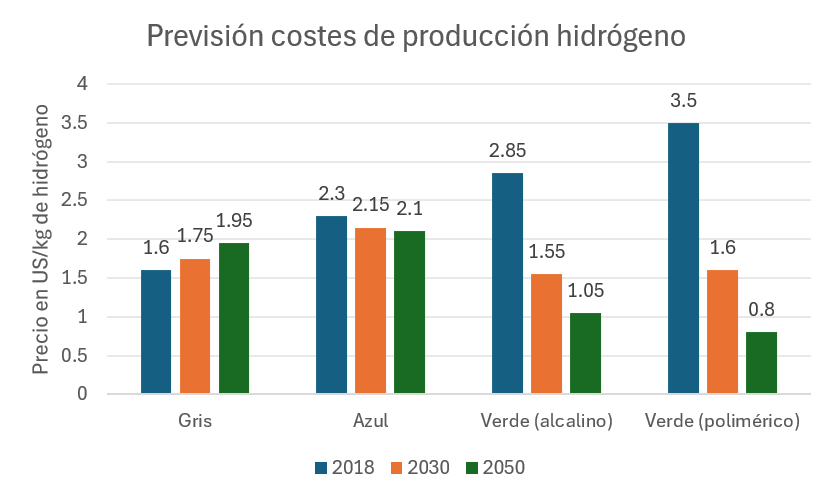
\includegraphics[width=0.7\linewidth]{res/tema3/hidrogeno1}
	\label{fig:hidrogeno1}
\end{figure}

\subsection{Ventajas del hidrógeno.}
\begin{itemize}
	\item [-]Aumenta la eficiencia y disminuir las emisiones en generación centralizada y
	distribuida.
	\item [-]Amortigua el carácter intermitente de los generadores renovables y aumentar la
	predictibilidad.
	\item [-]Permite la gestión de la carga.
	\item [-]Mejora la calidad de suministro: generación con pilas de combustible o motores de
	combustión.
\end{itemize}
\subsection{Aplicaciones del hidrógeno.}
Las principales aplicaciones son la pila de hidrógeno y la combustión directa del mismo en un motor.

La pila de hidrógeno se basa en una función redox en la cual al combinarse el hidrógeno con el oxígeno se forma agua, generando circulación de electrones. El principal inconveniente de estas baterías es que necesitan platino.
\begin{figure}[H]
	\centering
	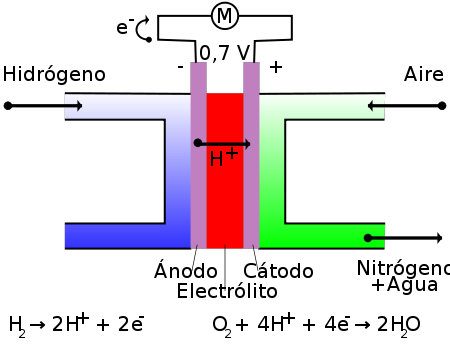
\includegraphics[width=0.68\linewidth]{res/tema3/hidrogeno2}
	\label{fig:hidrogeno2}
\end{figure}
Los motores de combustión, por su parte presentan eficiencias del 41,4\%.
\section{Ciclos combinados.}
Se trata de colocar en serie una turbina de gas natural que para enfriarlo se emplea vapor de agua que a su vez se hace pasar por una segunda turbina. Esto, permite mejorar la eficiencia del 36\% al 60\% y reducir el consumo de agua.
\begin{figure}[H]
	\centering
	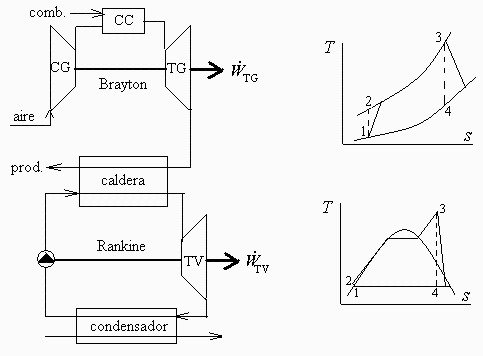
\includegraphics[width=0.7\linewidth]{res/tema3/ciclocombinao2}
	\label{fig:ciclocombinao2}
\end{figure}


\section{Fusión nuclear.}
La fusión nuclear consiste en una reacción donde dos núcleos ligeros se combinan para formar uno más pesado. La reacción más fácil de realizar es la del deuterio con el tritio:
\[H^2+H^3\rightarrow He^4 +n^1 + 17,6MeV\]

\begin{itemize}
	\item [-] \textbf{Deuterio:} Es un isótopo estable del hidrógeno formado por un protón y un neutrón. Hay 34g/m$^3$ de deuterio en el mar.
	\item [-]\textbf{Tritio:}  Es un isótopo inestable de hidrógeno formado por un protón y dos neutrones. Se desintegra con rapidez mediante radiación $\beta$. Se puede generar mediante reacciones de captura neutrónica con los isótopos del litio.
\end{itemize} 

Además, como el sistema no emplea materiales con elevada radiactividad no presenta el problema de los residuos nucleares de la fisión. No obstante, esta tecnología esta aún a nivel experimental y no existe ningún reactor comercial.
\section{Almacenamiento de energía.}
Los sistemas de almacenamiento de energía según su duración y número de usos tienen aplicaciones en la red distintas.
\begin{itemize}
	\item [-] \textbf{Calidad de energía:} Reacciona rápidamente aunque no tiene mucha autonomía. \underline{Supercondensadores}.
	\item [-] \textbf{Regulación primaria:} Reacciona con una velocidad similar a la anterior aunque se utiliza menos veces al día. \underline{Volantes de inercia}. 
	\item [-] \textbf{Reserva de suministro:} Se usa pocas veces pero tiene gran autonomía. \underline{Baterías y aire comprimido}.
	\item [-] \textbf{Desplazamiento de la demanda:} Se emplea para cubrir la demanda en horas punta. \underline{Bombeo}.
\end{itemize}

\subsection{Volantes de inercia.}
Son equipos giratorios que convierten la energía eléctrica en energía cinética (en una masa rodante) y cuando el sistema lo requiere lo devuelve a la red como energía eléctrica. Los volantes de inercia desempeñan un papel importante en la regulación primaria al dar inercia a los generadores síncronos.
\subsection{Supercondensadores.}
Es un dispositivo con un principio de funcionamiento similar al de un condensador tradicional pero con mayor capacidad y corriente de descarga. Tienen periodos de carga y descarga muy cortos lo que los hace apropiados para responder ante interrupciones del suministro de corta duración.
\subsection{Baterías.}
Es un dispositivo electroquímico que transforma la energía química en eléctrica. Su principal inconveniente es su coste, su alto volumen y su vida útil.
\subsection{Centrales de bombeo.}
En periodos valle en las centrales hidráulicas se bombea agua de la parte inferior del embalse de tal forma que se almacena la energía eléctrica en forma de energía potencial. \textbf{Actualmente e la única tecnología rentable} a nivel de almacenamiento en grandes cantidades.
\subsection{Aire comprimido (CAES).}
El almacenamiento es similar al almacenamiento por bombeo. El aire se comprime y se almacena en depósitos subterráneos y en periodos de demanda punta se libera expandiendo el aire a través de una turbina. Hoy en día solo existen dos plantas en el mundo.